\documentclass{article}
\usepackage[utf8]{inputenc}
\usepackage{amsmath}
\usepackage{amssymb}
\usepackage{float}
\usepackage{graphicx}
\usepackage{anysize}
\usepackage{amsthm}
\usepackage{marvosym}

% Controla los márgenes {izquierda}{derecha}{arriba}{abajo}. 
\marginsize{1.8cm}{1.5cm}{2cm}{3cm}
\renewcommand{\figurename}{Figura}

\title{\textsc{\Large{Métodos computacionales - Tarea 3}}}
\author{\textsc{\Large{Diego Gomez}}\hspace{10pt}(201318237)}
\date{}

\begin{document}

    \maketitle

    \begin{figure}[h]
        \centering
        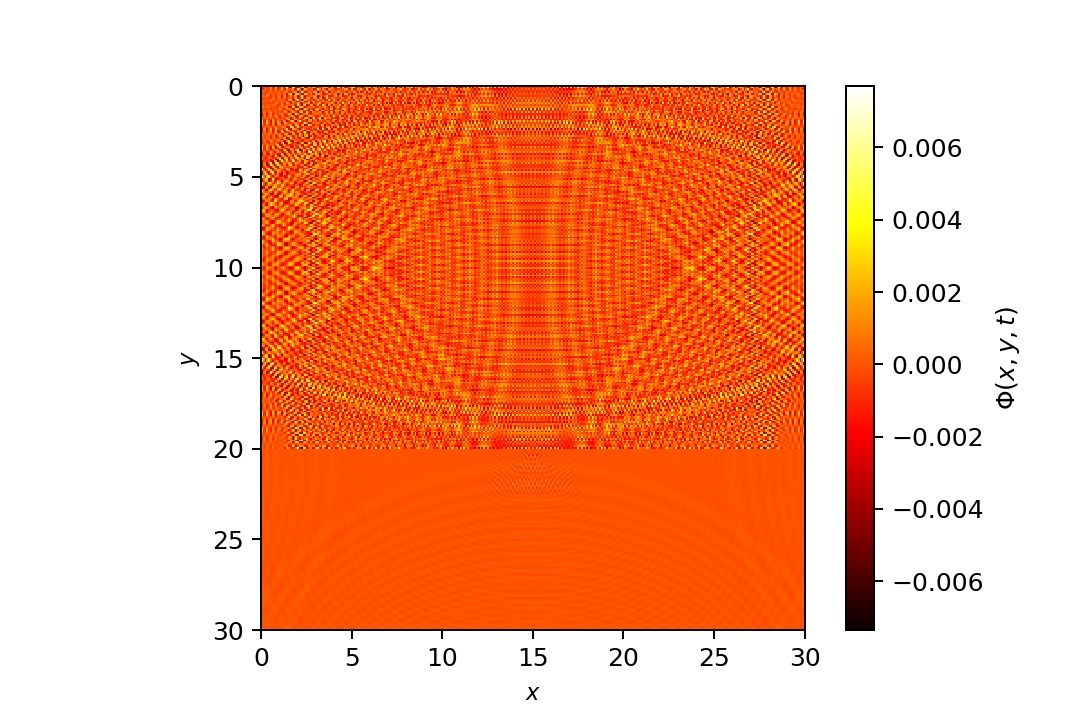
\includegraphics[width=0.55\textwidth]{Onda30.jpeg}
        \caption{Onda para $t=30$.}
        \label{fig:o30}
    \end{figure}
    
    \begin{figure}[h]
        \centering
        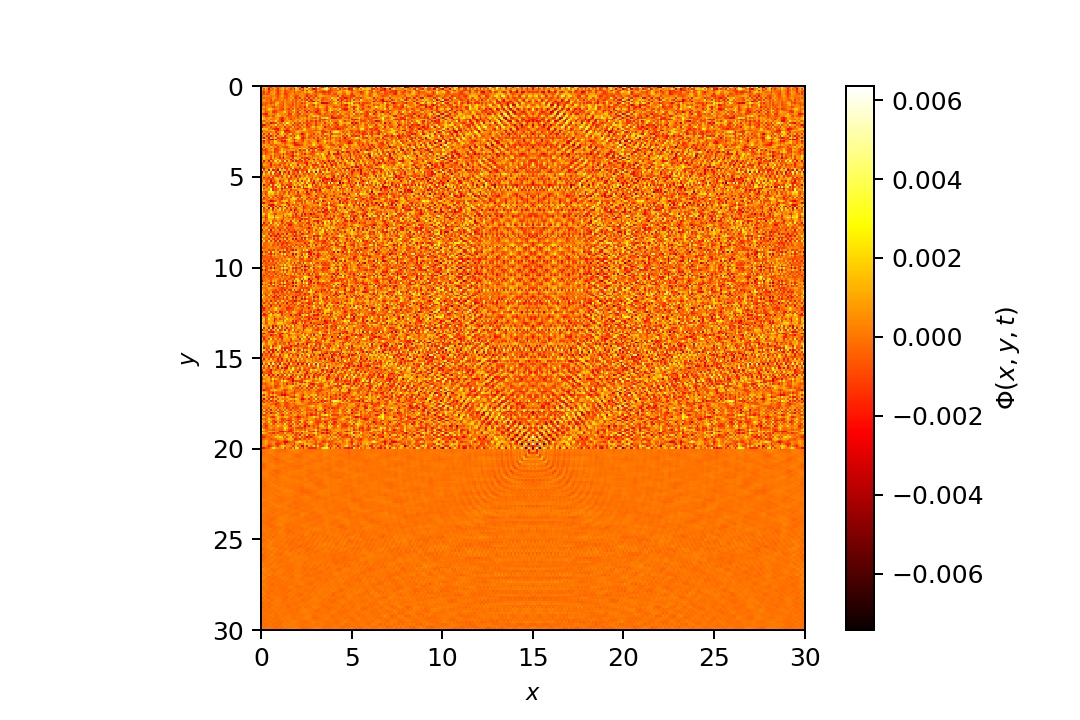
\includegraphics[width=0.55\textwidth]{Onda60.jpeg}
        \caption{Onda para $t=60$.}
        \label{fig:o60}
    \end{figure}

    \begin{figure}[h]
    	\centering
        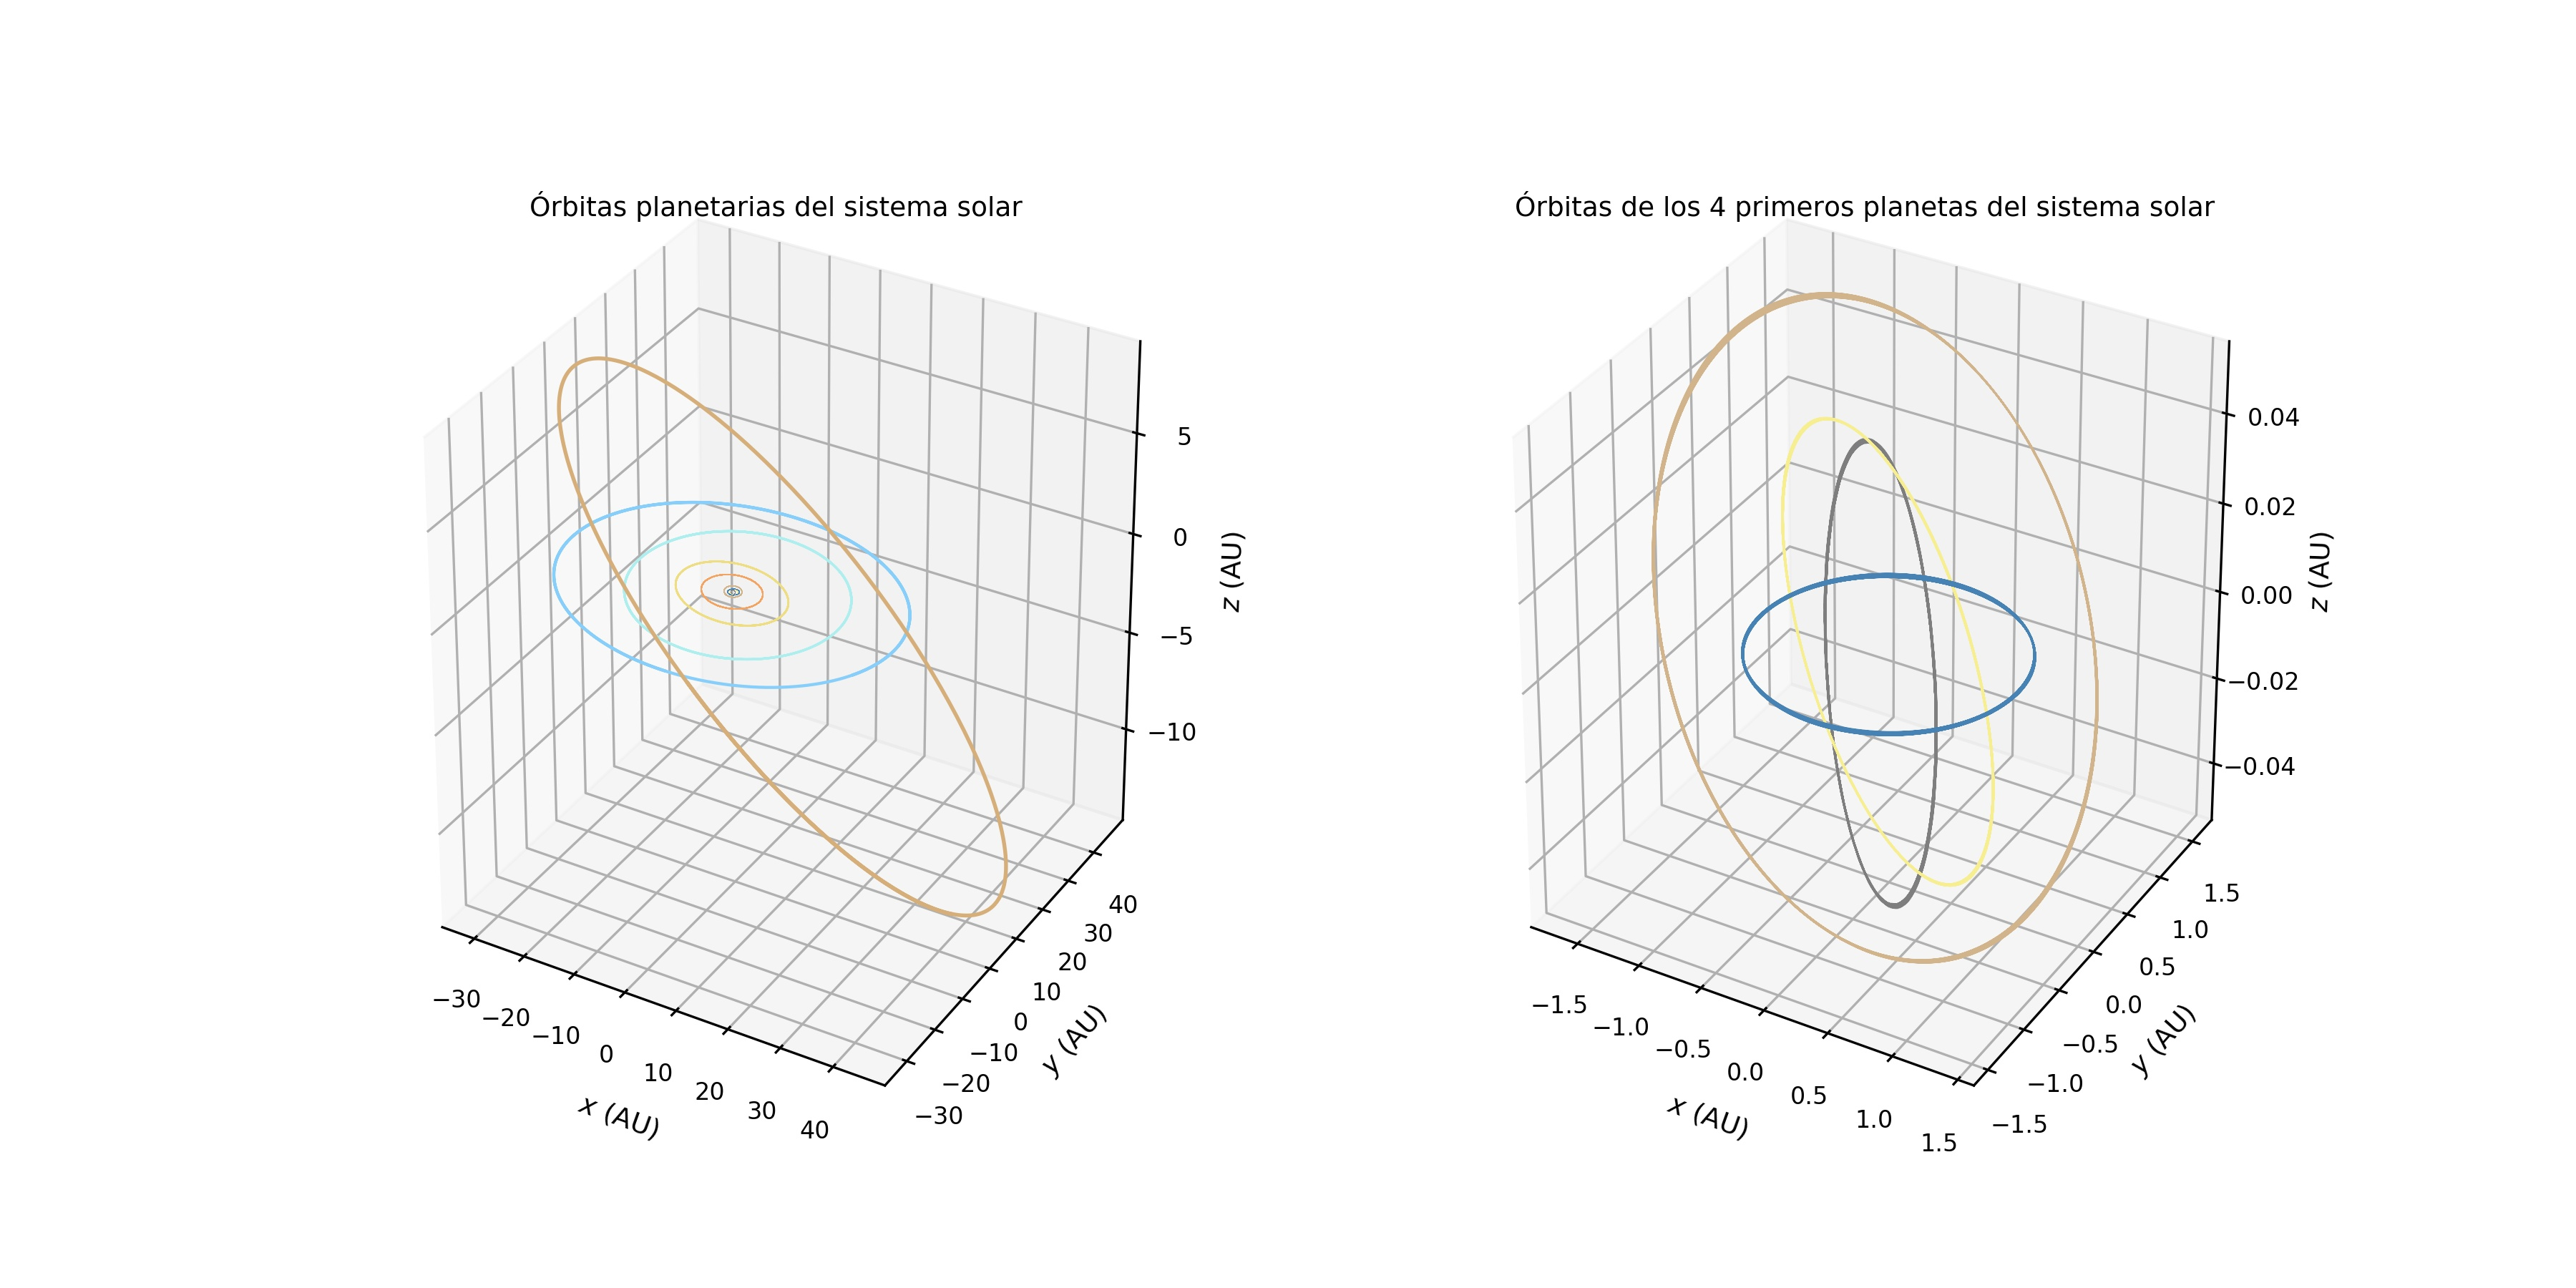
\includegraphics[width=\textwidth]{Planetas.jpeg}
        \caption{Órbitas de los planetas del sistema solar.}
        \label{fig:orb}
    \end{figure}    

\end{document}
